\section{Encoding} % Seções são adicionadas para organizar sua apresentação em blocos discretos, todas as seções e subseções são automaticamente exibidas no índice como uma visão geral da apresentação, mas NÃO são exibidas como slides separados.

%----------------------------------------------------------------------------------------

% \begin{frame}{Uniform PCM}
%     \begin{figure}
%         \centering
%         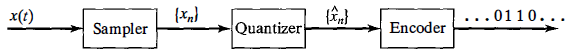
\includegraphics[width=0.7\linewidth]{img/PCM_steps.png}
%         %\caption{Block Diagram of a PCM System}
%         \label{fig:enter-label}
%     \end{figure}
%    \begin{align*}
%        \Delta = \frac{2x_{max}}{N} = \frac{x_{max}}{2^{\nu -1}}
%    \end{align*}
% \end{frame}

% %----------------------------------------------------------------------------------------
% \begin{frame}{$\mu$-law Compander}
%     \begin{figure}
%         \centering
%         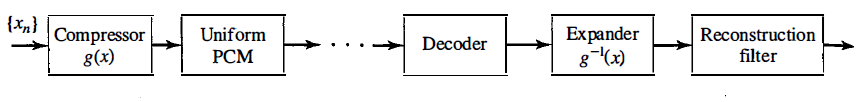
\includegraphics[width=0.7\linewidth]{img/non-unifor_PCM.png}
%         %\caption{Block Diagram of PCM}
%         \label{fig:block_pcm1}
%     \end{figure}
%     \begin{columns}

%          \column{0.48\textwidth}  % First column
%  \begin{figure}
%         \centering
%         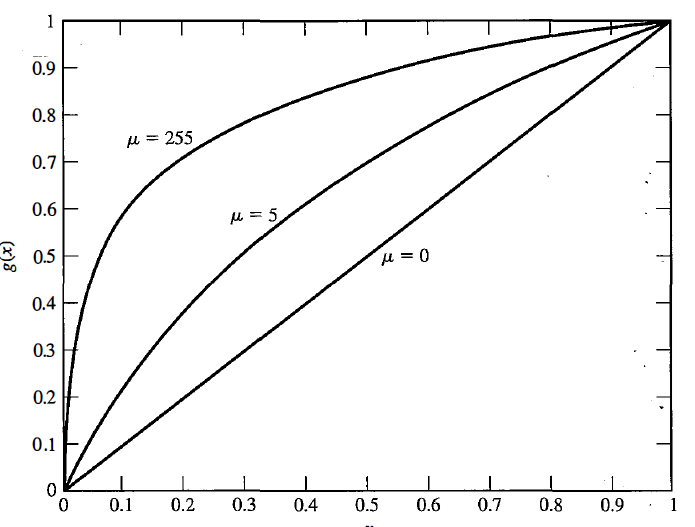
\includegraphics[width=1\linewidth]{img/mu-coding.png}
%         %\caption{Block Diagram of PCM}
%         \label{fig:u-law}
%     \end{figure}
%    \column{0.48\textwidth}  % First column
%     \begin{align*}
%        g(x) = \frac{\log (1+ \mu |x|)}{\log (1+\mu)} \text{sign}(x)
%    \end{align*}
%     \end{columns}
% \end{frame}

% %----------------------------------------------------------------------------------------
% \begin{frame}{A-law Compander}
%     \begin{figure}
%         \centering
%         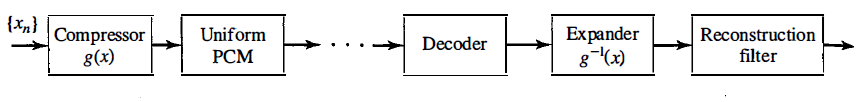
\includegraphics[width=0.7\linewidth]{img/non-unifor_PCM.png}
%         % \caption{Diagrama de blocos do PCM}
%         \label{fig:block_pcm}
%     \end{figure}
%        \begin{columns}

%          \column{0.48\textwidth}  % First column
%  \begin{figure}
%         \centering
%         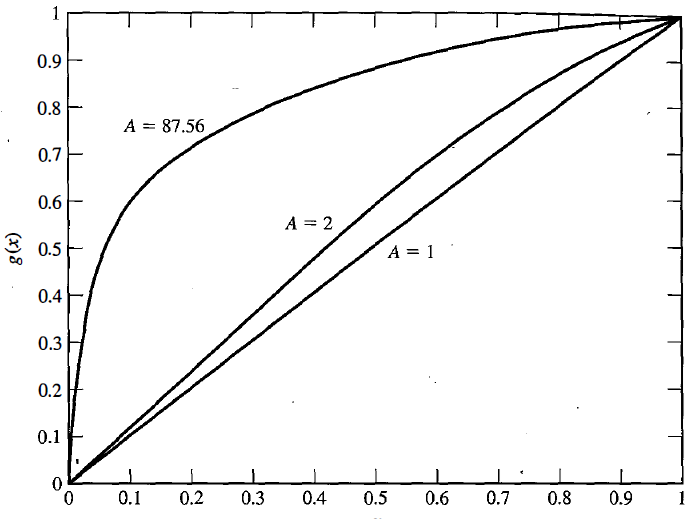
\includegraphics[width=1\linewidth]{img/A-coding.png}
%         % \caption{Diagrama de blocos do PCM}
%         \label{fig:a-law}
%     \end{figure}
%    \column{0.48\textwidth}  % First column
%     \begin{align*}
%        g(x) = \frac{1 +\log A |x|}{1 +\log A} \text{sign}(x)
%    \end{align*}
%     \end{columns}
% \end{frame}

%----------------------------------------------------------------------------------------